\documentclass[12pt]{article}
\usepackage{graphicx}
\usepackage{amsmath}
\usepackage{mathtools}

\newcommand{\mydet}[1]{\ensuremath{\begin{vmatrix}#1\end{vmatrix}}}
\providecommand{\brak}[1]{\ensuremath{\left(#1\right)}}
\providecommand{\norm}[1]{\left\lVert#1\right\rVert}
\newcommand{\solution}{\noindent \textbf{Solution: }}
\newcommand{\myvec}[1]{\ensuremath{\begin{pmatrix}#1\end{pmatrix}}}


\let\vec\mathbf
\begin{document}
\begin{center}
\textbf\large{CHAPTER-7 \\ COORDINATE GEOMETRY}

\end{center}
\section*{Excercise 7.4}

Q4.The two opposite vertices of a square are $(–1, 2) \text{ and } (3, 2)$. Find the coordinates of the other two vertices.\\
\textbf{Solution :}

Given points 
\begin{align*}
\vec{A} = \myvec
{
-1 \\
 2\\
},
\vec{C} = 
\myvec
{
3\\
2\\
}
\end{align*}

\begin{figure}[!h]
	\begin{center} 
	    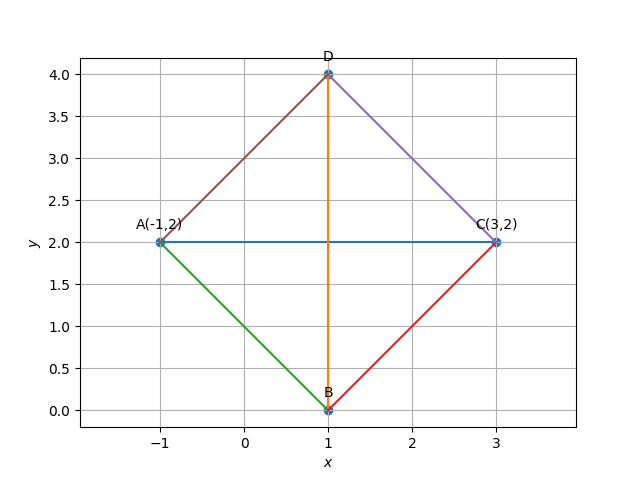
\includegraphics[width=\columnwidth]{./square}
	\end{center}
\caption{}
\label{fig:Fig1}
\end{figure}

Shifting point A to origin with refrence to Figure \ref{fig:Fig2}

\begin{align*}
\vec{A'} =
\myvec{
0 \\
0\\
},
\vec{C'} = \vec{C}-\vec{A} = 
\myvec{
4 \\
0\\
}
\end{align*}

\begin{figure}[!h]
	\begin{center} 
	    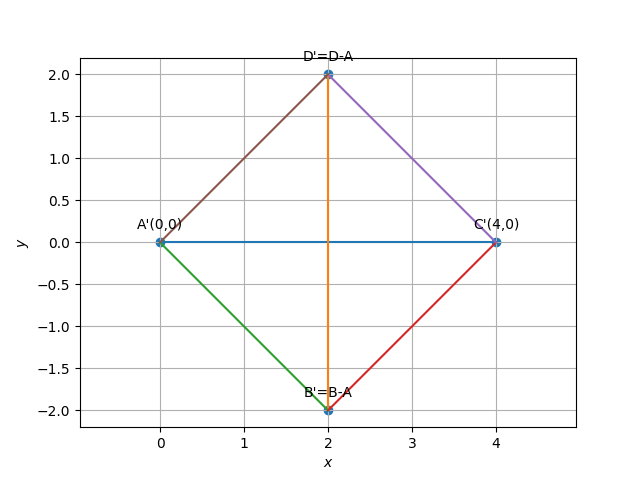
\includegraphics[width=\columnwidth]{./square1}
	\end{center}
\caption{}
\label{fig:Fig2}
\end{figure}

\newpage

For a generalised case, the angle made by $\vec{AC}$ on the x-axis will be $\theta + 45^{\circ}$, where $\theta$ is the angle made by $\vec{AB}$ on the x-axis.
Hence, we can calculate the angle made by $\vec{AB}$ on the x-axis as.
\begin{align*}
tan(\theta+45) &= \text{slope of } \vec{AC}\\
\beta = \theta+45 &= tan^{-1}(\text{slope of } \vec{AC})
\end{align*}
However in this particular case, angle made by $\vec{AC}$ on the x-axis
\begin{align*}
tan\beta &= \frac{0-0}{4-0}\\
\beta &= 0^{\circ}
\end{align*}

Therefore, here $\theta = -45^{\circ}$

We know the rotation matrix for CW rotation is given as
\begin{align*}
P^\top =
\myvec{
cos\theta & sin\theta \\
-sin\theta & cos\theta \\
}
\end{align*}

Since the angle here is negative so ultimately the coordinates will be rotated in ACW direction. Now the transformed(rotated) coordinates are with refrence to Figure \ref{fig:Fig3}.
\begin{align*}
\vec{C"} = P(\vec{C}-\vec{A}) =
\myvec{
\frac{1}{\sqrt{2}} & -\frac{1}{\sqrt{2}} \\
\frac{1}{\sqrt{2}} & \frac{1}{\sqrt{2}}\\
}
\myvec{
4 \\
0\\
} = 
\myvec{
\frac{4}{\sqrt{2}} \\
\frac{4}{\sqrt{2}}\\
}
\end{align*}
\begin{align*}
\vec{B"} = \myvec{
 1&0\\
 0&0\\
}\vec{C"}=
\myvec{
 \frac{4}{\sqrt{2}}\\
 0\\
},
\vec{D"} = \myvec{
 0&0\\
 0&1\\
}\vec{C"}=
\myvec{
 0\\
 \frac{4}{\sqrt{2}}\\
} \text{ and }
\vec{A"} =
\myvec{
0 \\
0\\
}
\end{align*}

\begin{figure}[!h]
	\begin{center} 
	    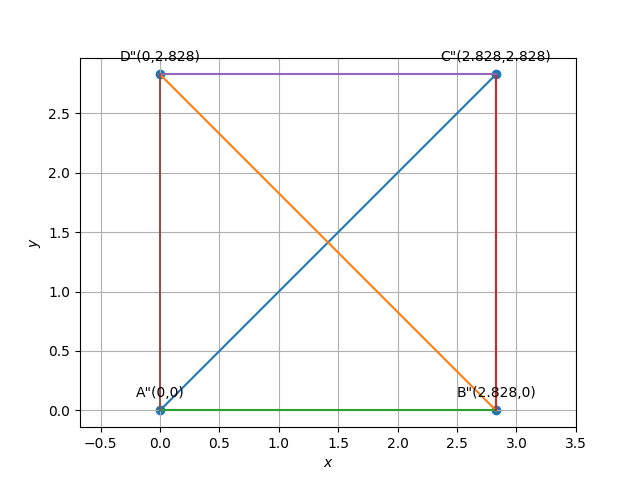
\includegraphics[width=\columnwidth]{./square2}
	\end{center}
\caption{}
\label{fig:Fig3}
\end{figure}

\newpage
Again tranforming(rotating) the coordinates back to the original axis.

We know for anti-clockwise direction the rotation matrix is given as
\begin{align*}
P =
\myvec{
cos\theta & -sin\theta \\
sin\theta & cos\theta \\
}
\end{align*}

Again we know that the angle is negative so the rotation will be in clockwise direction. So now the transformed(rotated) coordinates B and D are with refrence to Figure \ref{fig:Fig4}
\begin{align*}
\vec{B'} &= P\vec{B"} = \myvec{
\frac{1}{\sqrt{2}} & \frac{1}{\sqrt{2}} \\
-\frac{1}{\sqrt{2}} & \frac{1}{\sqrt{2}}\\
}
\myvec{
 \frac{4}{\sqrt{2}}\\
 0\\
} = 
\myvec{
2 \\
-2\\
}\\
\vec{D'} &= P\vec{D"} = \myvec{
\frac{1}{\sqrt{2}} & \frac{1}{\sqrt{2}} \\
-\frac{1}{\sqrt{2}} & \frac{1}{\sqrt{2}}\\
}
\myvec{
 0\\
 \frac{4}{\sqrt{2}}\\
} = 
\myvec{
2 \\
2 \\
}
\end{align*}

\begin{figure}[!h]
	\begin{center} 
	    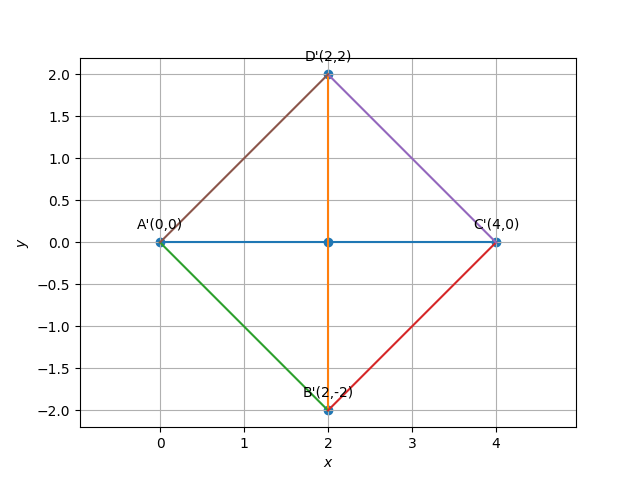
\includegraphics[width=\columnwidth]{./square3}
	\end{center}
\caption{}
\label{fig:Fig4}
\end{figure}

Again transforming(shifting) the axis back to the original with refrence to Figure \ref{fig:Fig5}
\begin{align*}
\vec{B} &= \vec{B'}+\vec{A} = \myvec{
2 \\
-2\\
}+\myvec{
-1 \\
2\\
} = 
\myvec{
1 \\
0\\
}\\
\vec{D} &= \vec{D'}+\vec{A} = \myvec{
2 \\
2\\
}+\myvec{
-1 \\
2\\
} = 
\myvec{
1 \\
4 \\
}
\end{align*}

Hence, the other two vertices are $\vec{B}(1,0) \text{ and } \vec{D}(1,4)$   

The direct formula for calculation of the vertices is:
\begin{align*}
\vec{B} &= \vec{A} + P[\vec{e_{1}}\text{ }\vec{0}]P^\top(\vec{C}-\vec{A})\\
\vec{D} &= \vec{A} + P[\vec{0} \text{ }\vec{e_{2}}]P^\top(\vec{C}-\vec{A})
\end{align*}

where $P$ is the rotation matrix and $\vec{A} \text{ and } \vec{C}$ are the position vectors of opposite vertices.

\begin{figure}[!h]
	\begin{center} 
	    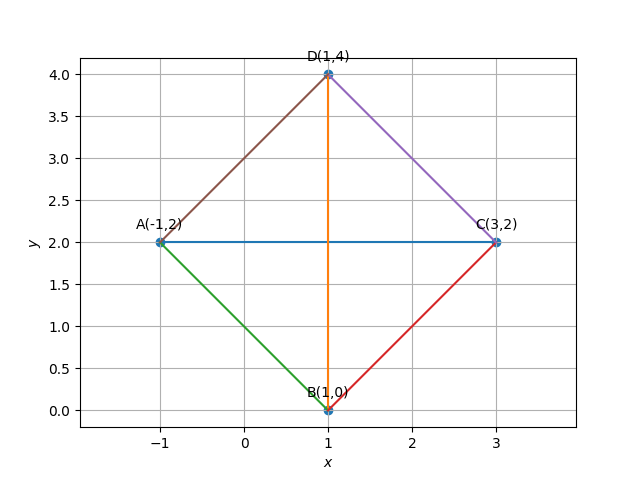
\includegraphics[width=\columnwidth]{./square4}
	\end{center}
\caption{}
\label{fig:Fig5}
\end{figure}





\end{document}